\documentclass[letterpaper,12pt]{article}
\usepackage{array}
\usepackage{threeparttable}
\usepackage{geometry}
\geometry{letterpaper,tmargin=1in,bmargin=1in,lmargin=1.25in,rmargin=1.25in}
\usepackage{fancyhdr,lastpage}
\pagestyle{fancy}
\lhead{}
\chead{}
\rhead{}
\lfoot{}
\cfoot{}
\rfoot{\footnotesize\textsl{Page \thepage\ of \pageref{LastPage}}}
\renewcommand\headrulewidth{0pt}
\renewcommand\footrulewidth{0pt}
\usepackage[format=hang,font=normalsize,labelfont=bf]{caption}
\usepackage{listings}
\lstset{frame=single,
  language=Python,
  showstringspaces=false,
  columns=flexible,
  basicstyle={\small\ttfamily},
  numbers=none,
  breaklines=true,
  breakatwhitespace=true
  tabsize=3
}
\usepackage{amsmath}
\usepackage{amssymb}
\usepackage{amsthm}
\usepackage{harvard}
\usepackage{setspace}
\usepackage{float,color}
\usepackage{graphicx}
\usepackage{hyperref}
\hypersetup{colorlinks,linkcolor=red,urlcolor=blue}
\theoremstyle{definition}
\newtheorem{theorem}{Theorem}
\newtheorem{acknowledgement}[theorem]{Acknowledgement}
\newtheorem{algorithm}[theorem]{Algorithm}
\newtheorem{axiom}[theorem]{Axiom}
\newtheorem{case}[theorem]{Case}
\newtheorem{claim}[theorem]{Claim}
\newtheorem{conclusion}[theorem]{Conclusion}
\newtheorem{condition}[theorem]{Condition}
\newtheorem{conjecture}[theorem]{Conjecture}
\newtheorem{corollary}[theorem]{Corollary}
\newtheorem{criterion}[theorem]{Criterion}
\newtheorem{definition}[theorem]{Definition}
\newtheorem{derivation}{Derivation} % Number derivations on their own
\newtheorem{example}[theorem]{Example}
\newtheorem{exercise}[theorem]{Exercise}
\newtheorem{lemma}[theorem]{Lemma}
\newtheorem{notation}[theorem]{Notation}
\newtheorem{problem}[theorem]{Problem}
\newtheorem{proposition}{Proposition} % Number propositions on their own
\newtheorem{remark}[theorem]{Remark}
\newtheorem{solution}[theorem]{Solution}
\newtheorem{summary}[theorem]{Summary}
%\numberwithin{equation}{section}
\bibliographystyle{aer}
\newcommand\ve{\varepsilon}
\newcommand\boldline{\arrayrulewidth{1pt}\hline}


\begin{document}

\begin{flushleft}
  \textbf{\large{Problem Set 4}} \\
  MACS 40000, Dr. Evans \\
  Sophia Mo
\end{flushleft}

\vspace{5mm}

\noindent\textbf{Problem 1(i)}\\
$\frac{\partial g_{cfe}(n)}{\partial n} = n^{\frac{1}{\sigma}}$\\
\\
$\frac{\partial g_{elp}(n)}{\partial n} = \frac{b}{\tilde{l}}(\frac{n}{\tilde{l}})^{\upsilon - 1}(1 - (\frac{n}{\tilde{l}})^\upsilon)^{\frac{1-\upsilon}{\upsilon}}$\\
\\
\noindent\textbf{Problem 1(ii)}\\
The estimated b is 0.5267708068873399, and upsilon is 1.4968180152979402.\\
\begin{center}
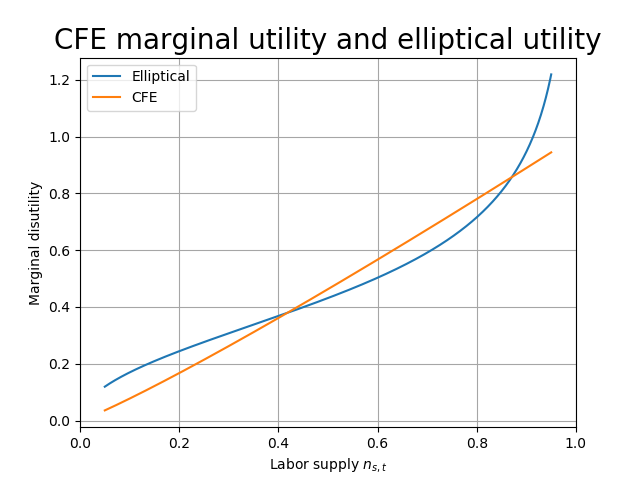
\includegraphics[scale=0.5]{Marginal_Disutility_ellip}
\end{center}
\\
\noindent\textbf{Problem 2(i)}\\
The marginal utility values obstained from the stitched function are:\\
1.40829679e+11,   5.75433098e+10,   4.59479342e+00,   1.22196463e-01\\
\begin{center}
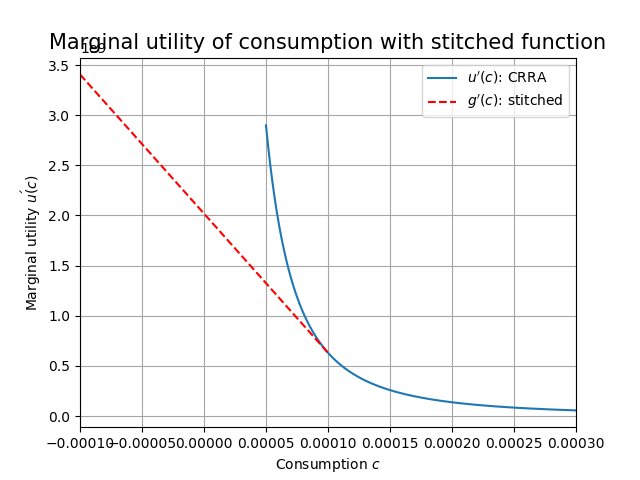
\includegraphics[scale=0.5]{MU_c_stitched}
\end{center}
\noindent\textbf{Problem 2(ii)}\\
The marginal disutility values are:\\
-3.24975000e+00,  -4.99750001e-01,   3.60237454e-01,   1.01976045e+05,
   1.60214791e+05\\
\begin{center}
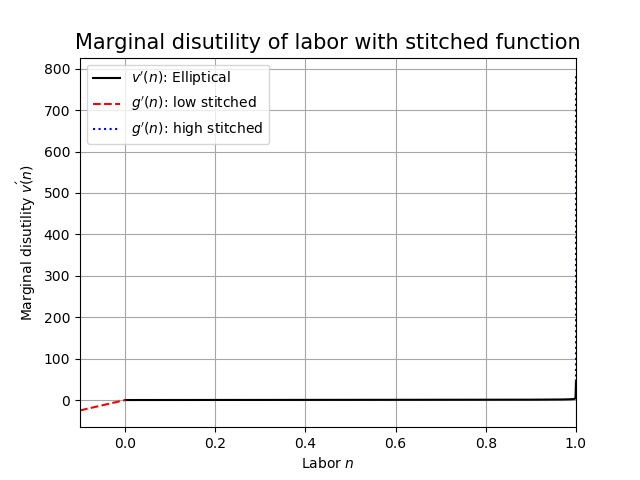
\includegraphics[scale=0.5]{MU_n_stitched}
\end{center}
\end{document}
